\begin{figure}[!h]
\setlength{\unitlength}{\textwidth}

  \begin{picture}(1,0.36)(0,0.74)
    
  \put(0.2,0.76){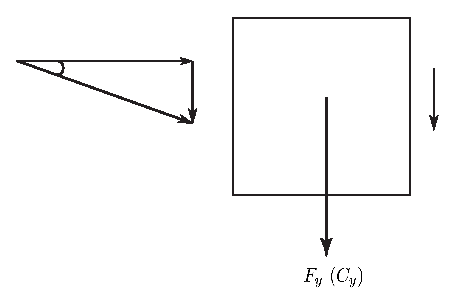
\includegraphics[width=0.5\unitlength]{./chapter-literature-revirw/fnp/setup-1.eps}}         
      
      
   
 	\put(0.315,1.04){$U$}
 	\put(0.3,0.95){$U_i$}
    \put(0.42,1.0){$\dot{y}$}
    \put(0.28,1.003){ $\theta$}
    \put(0.7,0.99){\small $(+)$}
      	

 	
 	 

     

  \end{picture}

 \caption{Induced angle of attack on a square prism due to the resultant of free-stream velocity of the fluid and transverse velocity of the body.}
    \label{fig:induced_lift_sketch}
\end{figure}